% MEMBRANE manuscript -- single-file LaTeX source.
%
% Compiles with a plain `pdflatex main.tex` (run 2-3 times for
% citations/references to settle -- paper/build.sh runs 3 passes and
% checks only the final pass's log, confirmed correct against a real
% GitHub Actions build) -- uses an inline `thebibliography`
% environment, not bibtex/biber, specifically so this file has no
% external bibliography-tool dependency. Uses the generic `article`
% class deliberately: no specific conference template is copied here
% because this project has not confirmed any single venue's template
% license/access terms yet -- see paper/submission-options.md. Once a
% venue is chosen, swap `\documentclass{article}` for that venue's own
% template and re-run paper/build.sh.
%
% Author/anonymous mode: set \anonymousfalse for the normal (authored)
% version, \anonymoustrue to strip the author block for anonymous
% review. Default: author mode (false).
\documentclass[11pt]{article}

\usepackage[utf8]{inputenc}
\usepackage[T1]{fontenc}
\usepackage[margin=1in]{geometry}
\usepackage{amsmath,amssymb}
\usepackage{graphicx}
\usepackage{booktabs}
\usepackage{hyperref}
\usepackage{xcolor}

\newif\ifanonymous
\anonymousfalse % default: author mode. Set \anonymoustrue for blind review.

\title{MEMBRANE: A Mixed-Precision, Exact-Retrieval Architecture for LLM KV-Cache Memory}
\ifanonymous
  \author{Anonymous Author(s)}
\else
  \author{Kadir Eren Altınta\c{s}}
\fi
\date{}

\begin{document}
\maketitle

\begin{abstract}
LLM inference servers are typically compute-rich but memory-poor:
KV-cache size grows linearly with context length and concurrent request
count, and full-attention traffic and classic PCIe-based offload latency
both become binding constraints before compute does. We present
MEMBRANE, a research prototype exploring whether a per-block memory
decision engine -- combining precision tiering and exact
(non-approximate) retrieval -- can reduce KV-cache memory traffic
without degrading retrieval quality, and where such a design does not
help. MEMBRANE combines a runtime-calibrated mixed-precision KV-cache
tier (FP16/Q8/Q4, verified bit-exact against ggml's reference
quantizer), an exact sparse KV retrieval engine (predictor, prefetch,
and a compulsory-miss fetch that is never approximated), a
discrete-event near-memory/CXL appliance simulator calibrated from real
captured attention traces, and a synthesizable FPGA quantization
datapath cosimulated against the same CPU reference math. Across a
unified 128K-context $\times$ 512-concurrency discrete-event stress
sweep (462/462 scenarios, two open SmolLM2 checkpoints), we measure
187x--405x KV-traffic reduction against a full-scan-CXL baseline and a
520{,}000-transaction, zero-mismatch Verilator cosimulation of the FPGA
datapath against its CPU reference. We also report, without suppressing
them, five null/negative findings: blind lossless compression fails on
real KV-cache data; PCIe-round-trip FPGA quantization offload is a net
loss at live-decode batch sizes; naive approximate KV eviction breaks
recall-shaped prompts; a 10ms p99 latency target is not met in any of
the 462 real scenarios, bounded by each model's own decode compute floor
rather than retrieval quality; and micro-batching shows no measurable
benefit at calibrated real demand levels. MEMBRANE remains a
simulation-heavy research prototype: no physical CXL or FPGA hardware
was used, and every hardware-adjacent number is either a cosimulation, a
synthesis-level check, or an explicit, cited assumption.
\end{abstract}

\section{Introduction}

Large language model inference servers are, in practice, often
memory-bound rather than compute-bound at serving time. Three cost
sources compound as context length and concurrent request count grow:
(1) \emph{KV-cache capacity} grows linearly per sequence and multiplies
across concurrent requests, so GPU memory capacity -- not FLOPs -- is
often what runs out first \cite{kwon2023pagedattention,sheng2023flexgen};
(2) \emph{full-attention traffic cost} scales memory traffic per decode
step linearly with context length, which sparse/selective-attention
methods try to reduce by different means
\cite{zhang2023h2o,xiao2024streamingllm,tang2024quest}; (3)
\emph{classic PCIe offload latency} trades capacity for a real
per-transfer cost that offloading systems must amortize carefully
\cite{sheng2023flexgen,lee2024infinigen} -- and, as this paper's own
hardware-in-the-loop measurement shows (RQ4, \S\ref{sec:eval}), that
cost can make small-batch FPGA-based offload a net loss. This motivates
(4) an explicit memory-tier / near-memory design, in the spirit of
recent CXL-attached near-memory processing proposals
\cite{xie2025trace,kim2025pnmcxl}.

MEMBRANE's research question is narrower than ``build a faster
KV-cache'': \emph{for a real KV access pattern captured from actual
inference, does a decision engine that tiers precision and retrieves
exactly -- rather than approximately -- measurably reduce memory
traffic without degrading retrieval quality, and at what latency cost?
And where does this design not help?} \S\ref{sec:eval} and
\S\ref{sec:negative} answer both halves honestly, with every headline
number traceable to a committed artifact (\texttt{benchmarks/MANIFEST.json}).

\paragraph{Contributions.} This paper makes five contributions, each
stated at the scope it can actually support (full comparison:
\texttt{paper/related-work-matrix.md}):
\begin{enumerate}
\item A runtime-calibrated, hot/warm/cold KV-cache tiering policy over
  FP16/Q8/Q4 precision, with the quantize/dequantize path verified
  bit-exact against ggml's own reference implementation across
  100{,}000+ randomized blocks plus every disclosed edge case.
\item A synthesizable FPGA quantization datapath sharing the identical
  bit-exact arithmetic as the CPU reference, cosimulated in Verilator
  across 520{,}000 transactions with zero mismatches -- to our
  knowledge, among the surveyed FPGA-quantization and CXL near-memory
  literature, none report this specific CPU/RTL bit-exact-parity
  verification methodology at this transaction count.
\item A disclosed, quantified negative result on PCIe-round-trip FPGA
  quantization-offload economics at live-decode batch sizes, derived
  from a real hardware-in-the-loop timing model.
\item An exact (non-approximate) sparse KV retrieval architecture for a
  simulated CXL/near-memory tier, distinguished from eviction-based
  \cite{zhang2023h2o,liu2023scissorhands,xiao2024streamingllm} and
  selection-based \cite{tang2024quest,kim2025pnmcxl} prior art by never
  permanently excluding attended content.
\item A real, out-of-core discrete-event simulation and
  artifact-verification infrastructure that completed a unified
  128K-context $\times$ 512-concurrency stress sweep (462/462
  scenarios) on a memory-constrained (5.6\,GiB RAM) development
  machine, with every headline number automatically checked against its
  source artifact.
\end{enumerate}

\section{Background}

MEMBRANE's own empirical starting point is a negative one: byte-level
lossless compression does not work on real KV-cache tensors. Measured
Shannon entropy of real, captured F16 KV data from actual llama.cpp
inference is 7.3--7.4 bits/byte, independent of prompt content, block
size, or K-vs-V -- byte-level RLE achieves exactly 1.000x (every block
falls back to raw storage) and would expand the data to 0.502x without
that fallback. This result redirected this project toward quantization
rather than generic compression.

\section{System design}

MEMBRANE is a from-scratch C11/C++17 implementation, described here as
one coherent system. See \texttt{docs/architecture.md} for the four
accompanying diagrams this section follows (Figure~\ref{fig:arch}).

\begin{figure}[h]
\centering
\IfFileExists{figures/generated/system_architecture.pdf}{
  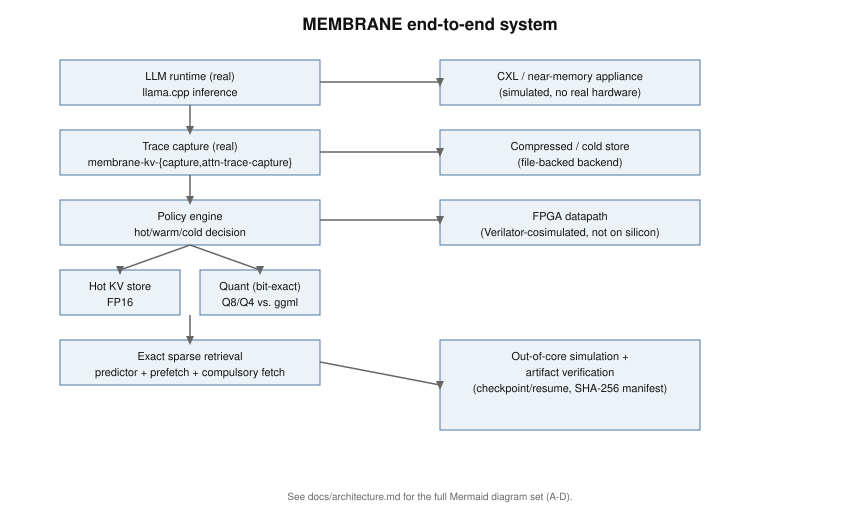
\includegraphics[width=0.85\textwidth]{figures/generated/system_architecture.pdf}
}{
  \fbox{\parbox{0.85\textwidth}{\centering Figure not available as PDF in
  this build environment (no SVG$\to$PDF converter found) -- see
  \texttt{paper/figures/generated/system\_architecture.svg}.}}
}
\caption{MEMBRANE end-to-end system: LLM runtime, real trace capture,
policy engine, hot/warm/cold KV tiers, exact sparse retrieval, simulated
CXL/near-memory appliance, cosimulated FPGA datapath, and the
out-of-core simulation/verification infrastructure.}
\label{fig:arch}
\end{figure}

\subsection{Block store and lossless baseline} A budget-aware block
store (\texttt{include/membrane/store.h}) with pluggable codecs and a
persistent file-backed cold tier. Its adaptive RAW fallback (never
expanding incompressible data) is what matters here, given
\S2's negative result.

\subsection{Mixed-precision (Q8/Q4) tiering} FP16 (hot) $\to$ Q8 (warm)
$\to$ Q4 (cold), promoted/evicted under a fixed byte budget, verified
bit-exact against ggml's Q8\_0/Q4\_0 reference across 100{,}000+
randomized blocks plus every disclosed edge case
(\texttt{tests/unit/test\_ggml\_quant\_parity.c}).

\subsection{Runtime-calibrated policy} Promotion/eviction thresholds are
calibrated against real runtime behavior, not fixed a priori -- this
process found and fixed a real decode-shape bug, and quantified that
quantize-function choice (not measurement noise) dominates the
offline-vs-runtime prediction gap.

\subsection{Exact sparse retrieval} A predictor estimates which blocks a
future attention step will need and issues a prefetch; every block
attention actually needs is exactly fetched on a compulsory miss if not
already resident -- correctness is never approximated, only the
prefetch \emph{decision} is predicted.

\subsection{CXL / near-memory appliance simulation} A discrete-event
simulator modeling link/device/quant-engine queues with real simulated
contention, calibrated once from a real captured trace. No physical CXL
hardware exists in this project; link figures are cited, industry-typical
assumptions informed by the CXL Consortium's specification
\cite{cxlconsortium2023spec} and standard PCIe-generation bandwidth
figures, not a literal quote from either.

\subsection{FPGA datapath} A fully synthesizable, purely-integer
fixed-point Q8/Q4 encode/decode pipeline, confirmed to elaborate under
yosys~0.33, cosimulated in Verilator against the CPU reference for
520{,}000 transactions across all four modes plus a mixed-mode
interleave, zero mismatches. Not placed, routed, or run on physical
silicon.

\subsection{Out-of-core, memory-bounded infrastructure} The unified
128K$\times$512 sweep's largest runs exceed this 5.6\,GiB development
machine's RAM if held naively in memory. A chunked, checksummed
out-of-core trace format, a bounded LRU chunk cache, and a real
\texttt{/proc}-based memory guard let the full sweep complete without
raising the RAM ceiling.

\section{Methodology}

Every experiment belongs to exactly one class, named explicitly in every
results table: \emph{real inference}, \emph{real trace capture},
\emph{CPU benchmark}, \emph{RTL simulation (cosimulation)},
\emph{synthesis (not silicon)}, \emph{discrete-event simulation},
\emph{extrapolated long-context trace}, \emph{oracle analysis}, and
\emph{assumed hardware profile}. See \texttt{paper/main.md} \S4 for the
full table mapping each class to its examples in this paper.

\section{Evaluation}
\label{sec:eval}

Each research question states its experiment, result, interpretation,
and limitation, with experiment class named. Full sourcing:
\texttt{paper/claim-audit.md}.

\begin{table}[h]
\centering
\small
\begin{tabular}{@{}lrrrr@{}}
\toprule
Comparison & 135M bytes/token & 135M reduction & 360M bytes/token & 360M reduction \\
\midrule
exact-no-prefetch          & 4{,}722{,}553  & 321.1x & 6{,}660{,}908  & 404.7x \\
exact-predictor            & 4{,}722{,}553  & 321.1x & 6{,}660{,}908  & 404.7x \\
exact-predictor-prefetch   & 8{,}100{,}157  & 187.2x & 11{,}008{,}426 & 244.9x \\
exact-predictor-coalescing & 8{,}100{,}157  & 187.2x & 11{,}008{,}426 & 244.9x \\
oracle                     & 4{,}722{,}849  & 321.1x & 6{,}661{,}085  & 404.7x \\
\bottomrule
\end{tabular}
\caption{Major results at the representative 8GiB-host/2TiB-device/all-Q8
point. ``Reduction'' is vs. the full-scan-CXL analytical baseline.
Source: \texttt{benchmarks/cxl-sim/unified-sweep.csv}; regenerated by
\texttt{paper/scripts/generate-tables.py} (\texttt{paper/tables/major-results.md}).}
\label{tab:major-results}
\end{table}

\textbf{RQ1 (capacity):} Lossless compression recovers 0x additional
capacity on real KV data. Q8/Q4 tiering pushes
\texttt{cap\_effective\_capacity\_ratio} above 1.0 at the 2TiB device
point for SmolLM2-135M, but SmolLM2-360M's fp16 tier never reaches 1.0
even at 2TiB (0.7998) -- capacity accounting is simulated/analytical,
not measured against a real device.

\textbf{RQ2 (quality):} Quantize/dequantize is bit-exact (0 mismatches,
100{,}000+ blocks); end-to-end quality is measured against real
inference on both models, at 135M/360M scale (far below production LLM
sizes).

\textbf{RQ3 (FPGA parity):} 520{,}000 transactions, 0 mismatches
(Table~\ref{tab:hw-verification}) -- a cosimulation result, not a
silicon result.

\begin{table}[h]
\centering
\small
\begin{tabular}{@{}lll@{}}
\toprule
Verification & Method & Result \\
\midrule
FPGA vs. CPU reference & Verilator cosimulation & 520{,}000 tx, 0 mismatches \\
CPU quantizer vs. ggml & Direct linked comparison & 100{,}000+ blocks, 0 mismatches \\
RTL synthesizability & yosys 0.33 elaboration & elaborates cleanly \\
\bottomrule
\end{tabular}
\caption{Hardware datapath verification. Source: \texttt{rtl/tb/tb\_top\_verilator.cpp},
\texttt{tests/unit/test\_ggml\_quant\_parity.c}.}
\label{tab:hw-verification}
\end{table}

\textbf{RQ4 (PCIe offload):} A real PCIe round trip of even 1--2
microseconds would make per-block/small-batch FPGA offload a net loss
versus CPU-only quantization (real per-block cost: 20--180ns) -- a
composed, disclosed, not-on-real-hardware conclusion.

\textbf{RQ5 (near-memory retrieval):} 187x--405x reduction vs.
full-scan-CXL at the representative point (99.6x--215.3x vs. a
compressed baseline); a separate 4K-context scenario shows
985.7x--1{,}281.1x (never conflated with the 128K figure). Oracle and
real-predictor bytes/token differ by under 0.01\% per model.

\textbf{RQ6 (128K$\times$512 behavior):} 462/462 scenarios complete
(Table~\ref{tab:unified-stress}); p99 never meets a 10ms illustrative
bound in any real scenario, for either model.

\begin{table}[h]
\centering
\small
\begin{tabular}{@{}lrrrl@{}}
\toprule
Model & Total rows & Real rows & 10ms p99 met & Capacity $\geq$1.0 (any device, Q8) \\
\midrule
SmolLM2-135M & 231 & 225 & 0/225 & yes \\
SmolLM2-360M & 231 & 225 & 0/225 & yes \\
\bottomrule
\end{tabular}
\caption{Unified stress results. 462/462 total across both models.
Source: \texttt{benchmarks/cxl-sim/unified-sweep.csv}.}
\label{tab:unified-stress}
\end{table}

\textbf{RQ7 (bottleneck):} dropping quant-pipeline count 8$\to$1
inflates p99 by 25.7x (15.67ms $\to$ 402.1ms); CXL-3.0-class vs.
CXL-latency-low/med/high shows no measurable difference at the same
point. The model's own real decode compute floor (15.67ms/token for
135M, $\sim$41.0ms/token for 360M) alone already exceeds the 10ms bound.
\textbf{The quant-pipeline count and model compute floor dominate; CXL
link generation, at this scenario point, does not.} (135M-only by
original design.)

\section{Negative results}
\label{sec:negative}

Kept as a first-class, visible section (Table~\ref{tab:negative}) --
these are as scientifically load-bearing as \S\ref{sec:eval}'s positive
findings.

\begin{table}[h]
\centering
\small
\begin{tabular}{@{}p{0.55\textwidth}p{0.35\textwidth}@{}}
\toprule
Finding & Key number \\
\midrule
Blind lossless compression fails on real KV data & 1.000x (RAW fallback) \\
PCIe-round-trip FPGA offload is a net loss (small batches) & 1--2us RTT vs. 20--180ns CPU \\
Naive approximate KV eviction breaks recall-shaped tasks & as low as 0.04 top-1 match rate \\
10ms p99 bound not met, either model & 0/225 real rows per model \\
Micro-batching shows no measurable benefit & null result \\
\bottomrule
\end{tabular}
\caption{Negative-result summary. See \texttt{paper/claim-audit.md} for exact wording/source/limitation per row.}
\label{tab:negative}
\end{table}

\section{Limitations and threats to validity}

Small model scale (135M/360M, not 7B+); no real CXL hardware; no real
GPU serving-stack integration; trace extrapolation for 128K context; CPU
compute floor bounds all latency results; discrete-event simulator
assumptions (analytical queueing, not every real-hardware effect
modeled); no FPGA place-and-route or on-board result; limited
model/prompt diversity; Q4 quality risk not exhaustively characterized
across all deployment configurations; fixed top-k attention-trace
capture resolution. Full detail per item: \texttt{paper/main.md} \S7.

\section{Related work}

See \texttt{paper/related-work-matrix.md} for the full 12-column
comparison across 14 sources. \textbf{KV-cache eviction/heavy-hitter}:
H2O \cite{zhang2023h2o} and Scissorhands \cite{liu2023scissorhands}
evict low-importance tokens, real GPU results at 6.7B--30B scale;
MEMBRANE's exact retrieval never permanently discards attended content,
at the cost of not being validated at that scale or on real hardware.
\textbf{Attention sinks/sparse attention}: StreamingLLM
\cite{xiao2024streamingllm} and Quest \cite{tang2024quest}. \textbf{Paged
KV-cache management}: PagedAttention/vLLM \cite{kwon2023pagedattention}
-- the strongest real-hardware, real-concurrency result surveyed.
\textbf{Offloading/tiering}: FlexGen \cite{sheng2023flexgen} and
InfiniGen \cite{lee2024infinigen}, both on real GPU/CPU hardware.
\textbf{KV quantization}: KIVI \cite{liu2024kivi} and KVQuant
\cite{hooper2024kvquant}, both real-GPU, sub-4-bit. \textbf{Retrieval-aware
attention}: Landmark Attention \cite{mohtashami2023landmark}.
\textbf{CXL near-memory}: TRACE \cite{xie2025trace} and PNM-CXL
\cite{kim2025pnmcxl} (real-vs-simulated hardware status not
independently re-verified by this project). \textbf{FPGA quantization}:
F-BFQ \cite{haris2025fbfq} (real FPGA per its own abstract, a capability
MEMBRANE does not yet have).

\section{Ethics and artifact disclosure}

Model licenses: SmolLM2-135M/-360M-Instruct are real, public
HuggingFaceTB checkpoints, not redistributed by this project (see
\texttt{docs/licensing.md}). Trace privacy: all captured traces derive
from short, non-sensitive, project-authored prompts. Benchmark
generation: every cited artifact's generating command is recorded in
\texttt{benchmarks/MANIFEST.json}. Energy: no energy/power number
appears anywhere in this project. AI tool contribution policy: most of
this project's code, documentation, and manuscript text was drafted by
an AI coding agent (Claude Code) under Kadir Eren Altınta\c{s}'s
direction -- he set the architecture, experimental design, validation
criteria, and technical decisions, and reviewed every commit (see
\texttt{outreach/ai-assistance-disclosure.md}) -- \emph{[placeholder:
final disclosure wording pending venue selection, see
paper/submission-options.md]}. Authorship: Kadir Eren Altınta\c{s} is
the sole human author, project creator/lead/owner; no co-authors. This
is a claim about direction and ownership, not that every line was typed
by hand without AI assistance.

\section{Conclusion}

MEMBRANE demonstrates that a per-block precision-plus-exact-retrieval
decision engine, calibrated from real inference traces, measures real KV
traffic reductions at a meaningful combined scale (128K context, 512
concurrency) without approximating retrieval quality -- while equally
visibly demonstrating five places this specific design does not help.
MEMBRANE contributes a disclosed, bit-exact-verified, exact-retrieval
alternative to the eviction/selection-based mainstream of KV-cache
memory management, evaluated rigorously in simulation and at
CPU-benchmark scale, but not yet at the model scale, real-hardware
realism, or production-serving integration its closest prior art already
has.

\appendix
\section{Reproducibility statement}

\textbf{Commit:} recorded in \texttt{docs/phase7-academic-paper.md} and
\texttt{paper/scripts/verify-paper.py}'s output.
\textbf{Build flags:} \texttt{-DCMAKE\_BUILD\_TYPE=Release},
\texttt{-DMEMBRANE\_ENABLE\_LLAMA=ON} (ggml-parity build only),
\texttt{-DMEMBRANE\_ENABLE\_SANITIZERS=ON} / \texttt{-DMEMBRANE\_ENABLE\_TSAN=ON}
for verification builds.
\textbf{Model versions:} SmolLM2-135M-Instruct, SmolLM2-360M-Instruct
(F16 GGUF via \texttt{convert\_hf\_to\_gguf.py}).
\textbf{Trace formats:} \texttt{.kvtrace}, \texttt{.attntrace}/\texttt{.attntrace2},
\texttt{.attntrace3} (chunked, out-of-core).
\textbf{Environment:} this project's own development machine, 5.6\,GiB
RAM; gcc/clang, CMake $\geq$3.16, Verilator, yosys 0.33.
\textbf{Full commands:} \texttt{docs/reproduction.md} (3 levels),
\texttt{scripts/demo.sh} ($\sim$25--50s quick check, depending on cache state), \texttt{paper/build.sh}.
\textbf{Expected runtime/RAM/disk:} Level 1 $\sim$2--5 min; Level 2
$\sim$30--90 min; Level 3 multi-hour, $\sim$1--2\,GiB transient disk,
768\,MiB default memory budget.
\textbf{Checkpoint/resume:} JSONL checkpoint with trace/config-hash
staleness detection.
\textbf{Artifact hashes:} every cited artifact's SHA-256 in
\texttt{benchmarks/MANIFEST.json}.
\textbf{Known platform quirks:} ThreadSanitizer+ASLR interaction requires
\texttt{setarch \$(uname -m) -R} around the TSan run (not a data race);
Icarus Verilog 12.0 hangs on a specific Q8/Q4-decode-combined
simulation, worked around via Verilator.

% ---------------------------------------------------------------------
% Inline bibliography (thebibliography, not bibtex/biber) -- see the
% file header for why. Must stay in sync with paper/references.bib;
% paper/scripts/verify-paper.py checks paper/main.md's citations against
% references.bib, not this file, so any edit here should be mirrored
% there by hand.
% ---------------------------------------------------------------------
\begin{thebibliography}{99}

\bibitem{zhang2023h2o} Zhenyu Zhang, Ying Sheng, Tianyi Zhou, Tianlong Chen, Lianmin Zheng, Ruisi Cai, Zhao Song, Yuandong Tian, Christopher R\'e, Clark Barrett, Zhangyang Wang, Beidi Chen. H$_2$O: Heavy-Hitter Oracle for Efficient Generative Inference of Large Language Models. NeurIPS 2023. arXiv:2306.14048.

\bibitem{liu2023scissorhands} Zichang Liu, Aditya Desai, Fangshuo Liao, Weitao Wang, Victor Xie, Zhaozhuo Xu, Anastasios Kyrillidis, Anshumali Shrivastava. Scissorhands: Exploiting the Persistence of Importance Hypothesis for LLM KV Cache Compression at Test Time. NeurIPS 2023. arXiv:2305.17118.

\bibitem{xiao2024streamingllm} Guangxuan Xiao, Yuandong Tian, Beidi Chen, Song Han, Mike Lewis. Efficient Streaming Language Models with Attention Sinks. ICLR 2024. arXiv:2309.17453.

\bibitem{tang2024quest} Jiaming Tang, Yilong Zhao, Kan Zhu, Guangxuan Xiao, Baris Kasikci, Song Han. Quest: Query-Aware Sparsity for Efficient Long-Context LLM Inference. ICML 2024. arXiv:2406.10774.

\bibitem{kwon2023pagedattention} Woosuk Kwon, Zhuohan Li, Siyuan Zhuang, Ying Sheng, Lianmin Zheng, Cody Hao Yu, Joseph E. Gonzalez, Hao Zhang, Ion Stoica. Efficient Memory Management for Large Language Model Serving with PagedAttention. SOSP 2023. arXiv:2309.06180. DOI:10.1145/3600006.3613165.

\bibitem{sheng2023flexgen} Ying Sheng, Lianmin Zheng, Binhang Yuan, Zhuohan Li, Max Ryabinin, Daniel Y. Fu, Zhiqiang Xie, Beidi Chen, Clark Barrett, Joseph E. Gonzalez, Percy Liang, Christopher R\'e, Ion Stoica, Ce Zhang. FlexGen: High-Throughput Generative Inference of Large Language Models with a Single GPU. ICML 2023. arXiv:2303.06865.

\bibitem{lee2024infinigen} Wonbeom Lee, Jungi Lee, Junghwan Seo, Jaewoong Sim. InfiniGen: Efficient Generative Inference of Large Language Models with Dynamic KV Cache Management. OSDI 2024. arXiv:2406.19707.

\bibitem{liu2024kivi} Zirui Liu, Jiayi Yuan, Hongye Jin, Shaochen Zhong, Zhaozhuo Xu, Vladimir Braverman, Beidi Chen, Xia Hu. KIVI: A Tuning-Free Asymmetric 2bit Quantization for KV Cache. ICML 2024. arXiv:2402.02750.

\bibitem{hooper2024kvquant} Coleman Hooper, Sehoon Kim, Hiva Mohammadzadeh, Michael W. Mahoney, Yakun Sophia Shao, Kurt Keutzer, Amir Gholami. KVQuant: Towards 10 Million Context Length LLM Inference with KV Cache Quantization. NeurIPS 2024. arXiv:2401.18079.

\bibitem{mohtashami2023landmark} Amirkeivan Mohtashami, Martin Jaggi. Landmark Attention: Random-Access Infinite Context Length for Transformers. NeurIPS 2023. arXiv:2305.16300.

\bibitem{xie2025trace} Rui Xie, Asad Ul Haq, Yunhua Fang, Linsen Ma, Zirak Burzin Engineer, Liu Liu, Tong Zhang. TRACE: Unlocking Effective CXL Bandwidth via Lossless Compression and Precision Scaling. arXiv:2509.03377 (cs.AR), 2025.

\bibitem{kim2025pnmcxl} Dowon Kim, MinJae Lee, Janghyeon Kim, HyuckSung Kwon, Hyeonggyu Jeong, Sang-Soo Park, Minyong Yoon, Si-Dong Roh, Yongsuk Kwon, Jinin So, Jungwook Choi. Scalable Processing-Near-Memory for 1M-Token LLM Inference: CXL-Enabled KV-Cache Management Beyond GPU Limits. arXiv:2511.00321 (cs.AR), 2025.

\bibitem{haris2025fbfq} Jude Haris, Jos\'e Cano. F-BFQ: Flexible Block Floating-Point Quantization Accelerator for LLMs. LG-ARC Workshop @ ISCA 2025. arXiv:2510.13401.

\bibitem{cxlconsortium2023spec} CXL Consortium. Compute Express Link (CXL) Specification. CXL 3.1 (November 2023) / CXL 4.0. computeexpresslink.org.

\end{thebibliography}

\end{document}
